\section{Desgin}%
\label{sec:desgin}

\iffalse
这一张将写本系统是如何设计的,主要内容分为两部分:一部分是如何hook。另外一部分是如何实现对各种数据结构的保护。

本文的特权特指就是内存管理,管理VMCS的原因就是里边含有EPTP,其余的域并不进行保护。

那么文章的核心就是剥夺了VMM管理物理内存的权限,这就是HyperPS的P的内容。
那么针对这一特点,这一思路,设计要怎么写。
要说明如下的几个问题:1. 如何分离权限,即VMM管理内存都是靠什么实现的,特权的实现途径是啥,怎么将这些特权分离。这里要写出两个东西:1.1 原本的VMM对内存管理的相关函数被Hook,所有的操作都无法在VMM中实施,即完成了HOOK。1.2 为了防止攻击者直接修改EPT paging structure,这就是将EPT从常规的空间中移除。
这两个点要顺序换过来,先写移除,再写hook。
2. 第二要写怎么实现保护,在hook完成后,剥离了VMM对物理内存的管理,HyperPS是如何实现对内存的管理的。这里要假如关于缺页中断的相关内容,怎么处理EPT异常,也要处理新建EPT的内容,也要包括不同虚拟机的映射关系,也要绑定EPT与VM的关系,不允许VM和VMM更改EPTP内容。

上面的1 2就是两段的内容,首先要给出一个overview,讲整个框架的结构。

##################
开头内容中文初稿
##################
这一节,我们首先提出我们的HyperPS,我们详细描述HyperPS的构成组件。然后我们详细阐述了HyperPS是如何剥离原VMM对内存的管理权限的。最后我们提出HyperPS是如何实现对内存的保护,从而实现保护虚拟机的运行以抵御一个受危害的VMM。
讲HyperPS如何实现对物理内存的管理。
\fi
In this section, we first propose the architecture of HyperPS. Then, in the following subsection, we elaborate on how HyperPS stripped the compromised HostOS kernel's privilege of managing guest VM's memory and the physical memory. Finally, we propose how HyperPS manages the guest VM's memory and physical memory to resist the compromised HostOS/Hypervisor.


\subsection{HyperPS Overview}%
\label{sub:hyperps_overview}

% 首先一句话说明HyperPS要做什么,然后Figure depict the details on the architecture of HyperPS.
% As shown in Figure, 我们创造了一个同层隔离空间用于履行原本属于compromised HostOS的管理虚拟机物理内存的权力。


We present HyperPS to protect guest virtual machines against compromised hypervisor. In virtualization environment, the hyperivor deprivileges the guest VM’s kernel and interposes all interactions between guest VMs and the physical memory. Neither isolation between VMs nor virtual-physical mapping relationships in a VM will inevitable be tamperred if the hypervisor is compromised. HyperPS, thus, deprives the hypervisor of privileges on managing physical memory.


Figure \ref{fig:design} depicts the details on the architecture of HyperPS. 
Firstly, as shown in Figure \ref{fig:design}, we create a delicate kernel-level secure and isolated execution space, called HyperPS Space, to process privilege of managing physical memory that originally belonged to the compromised hypervisor. 
Funtions about physical management, such as EPT operations and EPTP switching operations in VMCS operations, are equivalently hooked into the HyperPS space. 
For cases where an attacker uses regular memory access or newly introduced malicious VMX assembly code to bypass the hooked functions and tamper with the relevant memory magement data structures, HyperPS removed VMCS and EPT, which are crucial to virtualization, from the original hypervisor space and places them in the HyperPS Space.
Secondly, in the HyperPS space, we introduce a new data structure, called Physical Page Tag Table (PPTT), to tag the mapping relations between the physical frames and the virtual machines. With the help of this data structure, even if an attacker tampers EPT Paging Structures with malicious value through a legal function, HyperPS can still effectively detect such attack and resist it.

%FIXME 图中的内容添加虚拟机退出的线,removed的字段加粗 pptt是表 修改成表的形式

\begin{figure}[htpb]
    \centering
    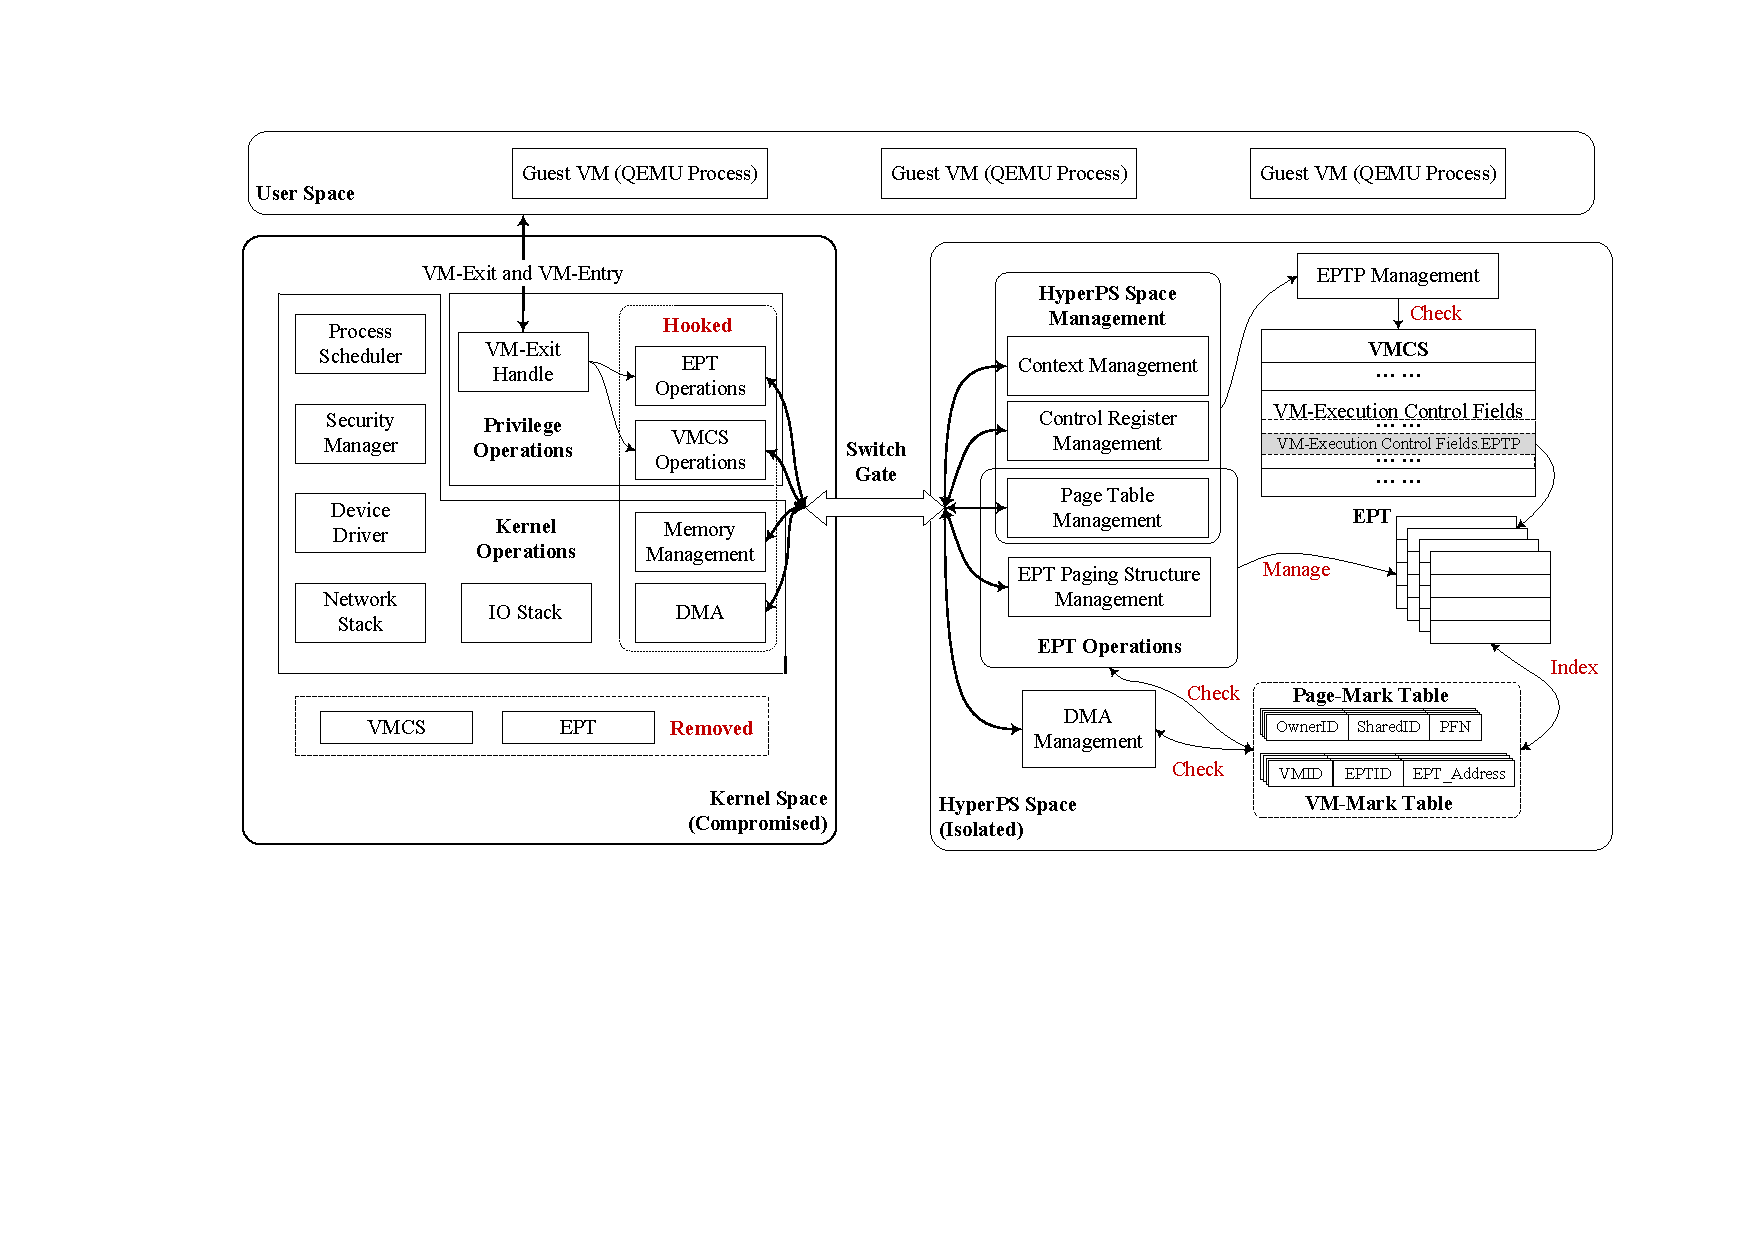
\includegraphics[width=0.9\linewidth]{IMG/design.pdf}
    \caption{HyperPS Architecture}%
    \label{fig:design}
\end{figure}


















